% Options for packages loaded elsewhere
\PassOptionsToPackage{unicode}{hyperref}
\PassOptionsToPackage{hyphens}{url}
\PassOptionsToPackage{dvipsnames,svgnames,x11names}{xcolor}
%
\documentclass[
  12pt,
]{article}

\usepackage{amsmath,amssymb}
\usepackage{setspace}
\usepackage{iftex}
\ifPDFTeX
  \usepackage[T1]{fontenc}
  \usepackage[utf8]{inputenc}
  \usepackage{textcomp} % provide euro and other symbols
\else % if luatex or xetex
  \usepackage{unicode-math}
  \defaultfontfeatures{Scale=MatchLowercase}
  \defaultfontfeatures[\rmfamily]{Ligatures=TeX,Scale=1}
\fi
\usepackage{lmodern}
\ifPDFTeX\else  
    % xetex/luatex font selection
    \setmainfont[]{Times New Roman}
\fi
% Use upquote if available, for straight quotes in verbatim environments
\IfFileExists{upquote.sty}{\usepackage{upquote}}{}
\IfFileExists{microtype.sty}{% use microtype if available
  \usepackage[]{microtype}
  \UseMicrotypeSet[protrusion]{basicmath} % disable protrusion for tt fonts
}{}
\usepackage{xcolor}
\usepackage[top=30mm,left=1in,right=1in,bottom=25mm]{geometry}
\setlength{\emergencystretch}{3em} % prevent overfull lines
\setcounter{secnumdepth}{5}
% Make \paragraph and \subparagraph free-standing
\makeatletter
\ifx\paragraph\undefined\else
  \let\oldparagraph\paragraph
  \renewcommand{\paragraph}{
    \@ifstar
      \xxxParagraphStar
      \xxxParagraphNoStar
  }
  \newcommand{\xxxParagraphStar}[1]{\oldparagraph*{#1}\mbox{}}
  \newcommand{\xxxParagraphNoStar}[1]{\oldparagraph{#1}\mbox{}}
\fi
\ifx\subparagraph\undefined\else
  \let\oldsubparagraph\subparagraph
  \renewcommand{\subparagraph}{
    \@ifstar
      \xxxSubParagraphStar
      \xxxSubParagraphNoStar
  }
  \newcommand{\xxxSubParagraphStar}[1]{\oldsubparagraph*{#1}\mbox{}}
  \newcommand{\xxxSubParagraphNoStar}[1]{\oldsubparagraph{#1}\mbox{}}
\fi
\makeatother


\providecommand{\tightlist}{%
  \setlength{\itemsep}{0pt}\setlength{\parskip}{0pt}}\usepackage{longtable,booktabs,array}
\usepackage{calc} % for calculating minipage widths
% Correct order of tables after \paragraph or \subparagraph
\usepackage{etoolbox}
\makeatletter
\patchcmd\longtable{\par}{\if@noskipsec\mbox{}\fi\par}{}{}
\makeatother
% Allow footnotes in longtable head/foot
\IfFileExists{footnotehyper.sty}{\usepackage{footnotehyper}}{\usepackage{footnote}}
\makesavenoteenv{longtable}
\usepackage{graphicx}
\makeatletter
\def\maxwidth{\ifdim\Gin@nat@width>\linewidth\linewidth\else\Gin@nat@width\fi}
\def\maxheight{\ifdim\Gin@nat@height>\textheight\textheight\else\Gin@nat@height\fi}
\makeatother
% Scale images if necessary, so that they will not overflow the page
% margins by default, and it is still possible to overwrite the defaults
% using explicit options in \includegraphics[width, height, ...]{}
\setkeys{Gin}{width=\maxwidth,height=\maxheight,keepaspectratio}
% Set default figure placement to htbp
\makeatletter
\def\fps@figure{htbp}
\makeatother
% definitions for citeproc citations
\NewDocumentCommand\citeproctext{}{}
\NewDocumentCommand\citeproc{mm}{%
  \begingroup\def\citeproctext{#2}\cite{#1}\endgroup}
\makeatletter
 % allow citations to break across lines
 \let\@cite@ofmt\@firstofone
 % avoid brackets around text for \cite:
 \def\@biblabel#1{}
 \def\@cite#1#2{{#1\if@tempswa , #2\fi}}
\makeatother
\newlength{\cslhangindent}
\setlength{\cslhangindent}{1.5em}
\newlength{\csllabelwidth}
\setlength{\csllabelwidth}{3em}
\newenvironment{CSLReferences}[2] % #1 hanging-indent, #2 entry-spacing
 {\begin{list}{}{%
  \setlength{\itemindent}{0pt}
  \setlength{\leftmargin}{0pt}
  \setlength{\parsep}{0pt}
  % turn on hanging indent if param 1 is 1
  \ifodd #1
   \setlength{\leftmargin}{\cslhangindent}
   \setlength{\itemindent}{-1\cslhangindent}
  \fi
  % set entry spacing
  \setlength{\itemsep}{#2\baselineskip}}}
 {\end{list}}
\usepackage{calc}
\newcommand{\CSLBlock}[1]{\hfill\break\parbox[t]{\linewidth}{\strut\ignorespaces#1\strut}}
\newcommand{\CSLLeftMargin}[1]{\parbox[t]{\csllabelwidth}{\strut#1\strut}}
\newcommand{\CSLRightInline}[1]{\parbox[t]{\linewidth - \csllabelwidth}{\strut#1\strut}}
\newcommand{\CSLIndent}[1]{\hspace{\cslhangindent}#1}

\usepackage{booktabs}
\usepackage{caption}
\usepackage{longtable}
\usepackage{colortbl}
\usepackage{array}
\usepackage{anyfontsize}
\usepackage{multirow}
\usepackage{sectsty}
\chapterfont{\centering}
\usepackage{lscape}
\newcommand{\blandscape}{\begin{landscape}}
\newcommand{\elandscape}{\end{landscape}}
\makeatletter
\@ifpackageloaded{caption}{}{\usepackage{caption}}
\AtBeginDocument{%
\ifdefined\contentsname
  \renewcommand*\contentsname{Table of contents}
\else
  \newcommand\contentsname{Table of contents}
\fi
\ifdefined\listfigurename
  \renewcommand*\listfigurename{List of Figures}
\else
  \newcommand\listfigurename{List of Figures}
\fi
\ifdefined\listtablename
  \renewcommand*\listtablename{List of Tables}
\else
  \newcommand\listtablename{List of Tables}
\fi
\ifdefined\figurename
  \renewcommand*\figurename{Figure}
\else
  \newcommand\figurename{Figure}
\fi
\ifdefined\tablename
  \renewcommand*\tablename{Table}
\else
  \newcommand\tablename{Table}
\fi
}
\@ifpackageloaded{float}{}{\usepackage{float}}
\floatstyle{ruled}
\@ifundefined{c@chapter}{\newfloat{codelisting}{h}{lop}}{\newfloat{codelisting}{h}{lop}[chapter]}
\floatname{codelisting}{Listing}
\newcommand*\listoflistings{\listof{codelisting}{List of Listings}}
\makeatother
\makeatletter
\makeatother
\makeatletter
\@ifpackageloaded{caption}{}{\usepackage{caption}}
\@ifpackageloaded{subcaption}{}{\usepackage{subcaption}}
\makeatother

\ifLuaTeX
  \usepackage{selnolig}  % disable illegal ligatures
\fi
\usepackage{bookmark}

\IfFileExists{xurl.sty}{\usepackage{xurl}}{} % add URL line breaks if available
\urlstyle{same} % disable monospaced font for URLs
\hypersetup{
  pdftitle={Power Acquisition and Leadership Survival: A Comparative Analysis of Coup-installed and Autocoup Leaders},
  pdfkeywords={Coups, Autocoups, Leadership Survival, Cox Model},
  colorlinks=true,
  linkcolor={blue},
  filecolor={Maroon},
  citecolor={Blue},
  urlcolor={blue},
  pdfcreator={LaTeX via pandoc}}


\title{Power Acquisition and Leadership Survival: A Comparative Analysis
of Coup-installed and Autocoup Leaders}
\author{}
\date{2024-10-15}

\begin{document}


\def\spacingset#1{\renewcommand{\baselinestretch}%
{#1}\small\normalsize} \spacingset{1}


%%%%%%%%%%%%%%%%%%%%%%%%%%%%%%%%%%%%%%%%%%%%%%%%%%%%%%%%%%%%%%%%%%%%%%%%%%%%%%

\date{2024-10-15}
\title{\bf Power Acquisition and Leadership Survival: A Comparative
Analysis of Coup-installed and Autocoup Leaders}
\author{
}

\maketitle

\bigskip
\bigskip
\begin{abstract}
This study examines the relationship between the methods of power
acquisition and the tenure of leaders who ascend to power through
unconventional means, with a particular focus on coup-installed and
autocoup leaders. The central hypothesis posits that the mode of
accession has a profound impact on leadership longevity. Utilizing Cox
proportional hazards and time-dependent Cox models, this study provides
robust empirical evidence of disparate survival times between these two
leader types. The findings reveal that, on average, coup-installed
leaders are 2.23 times more likely to be ousted from power than autocoup
leaders, all else being equal. These results have far-reaching
implications for political stability and democratic processes,
suggesting that the perceived low costs and high rewards associated with
autocoups may incentivize incumbents to prolong their tenure through
this means, potentially contributing to democratic erosion. This
research makes a notable contribution to the academic literature by
offering nuanced insights into the dynamics of irregular leadership
transitions and enhances our understanding of the complex interplay
between power acquisition methods and leadership longevity.
\end{abstract}

\noindent%
{\it Keywords:} Coups, Autocoups, Leadership Survival, Cox Model
\vfill

\newpage
\spacingset{1.9} % DON'T change the spacing!

\setstretch{1.618}
\section{Introduction}\label{introduction}

The enduring fascination with the longevity of political leaders has
sparked extensive research in political science, with scholars seeking
to understand why some leaders maintain power for decades while others
are ousted in a matter of months or even days. However, a specific
subset of leaders---those who ascend to power through coups or extend
their tenure through autocoups---has received relatively limited
attention. Examining the tenures of these leaders is crucial, as it
sheds light on the dynamics of irregular leadership transitions and
their implications for political stability and democratic processes.

In contrast to leaders who attain power through conventional means,
those who rise through irregular channels, such as coups or autocoups,
present more complex and intriguing cases for study. The Archigos
dataset highlights the prevalence of irregular power transitions.
Between 1945 and 2015, over half of leaders who assumed power
irregularly also exited irregularly, a rate significantly higher than
that of leaders who accessed office through regular channels.

Coup-installed and autocoup leaders constitute a substantial portion of
these irregular cases. The Archigos dataset notes that of 374 leaders
who exited irregularly, 246 (65.8\%) were ousted through coups.
Furthermore, research by Frantz and Stein
(\citeproc{ref-frantz2016}{2016}) demonstrates that coup-related exits
account for approximately one-third of all exits in autocracies,
surpassing any other transition type. Additionally, the autocoup
dataset, introduced by Zhu (\citeproc{ref-zhu2024}{2024}), documents 110
autocoup attempts between 1945 and 2023, of which 87 were successful.

Measuring the tenure of coup-installed and autocoup leaders poses
challenges due to the inherent irregularity and uncertainty of their
positions. Nevertheless, a comparative analysis reveals that leaders who
extend power through autocoups tend to have longer average post-autocoup
tenures (approximately 11 years) compared to coup-installed leaders
(approximately 5.7 years), suggesting a potential tenure gap of over
five years.

\begin{figure}

\centering{

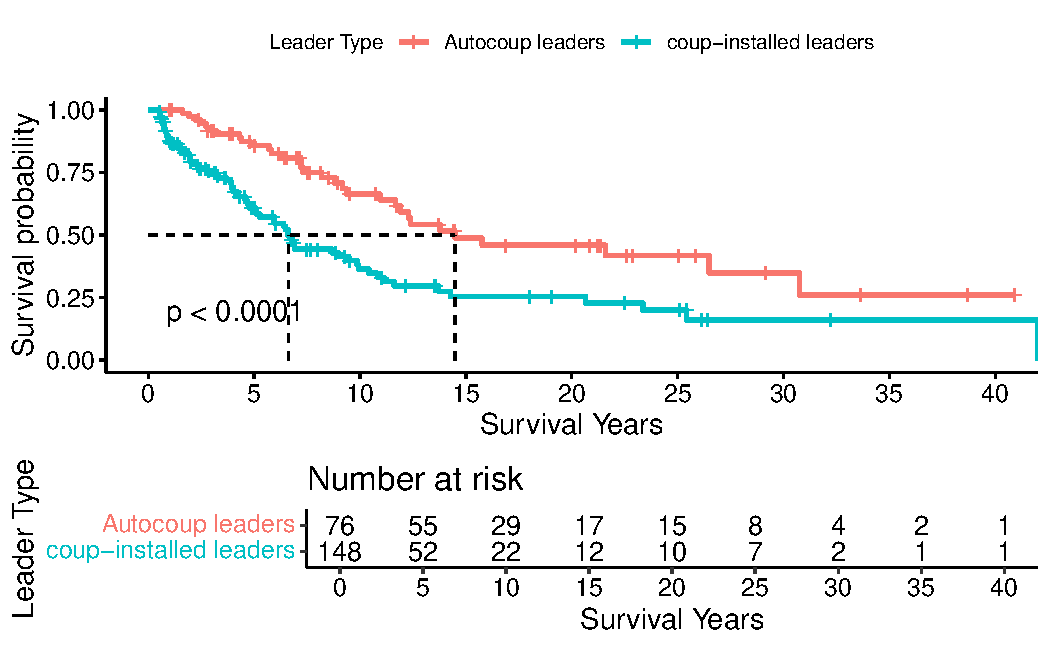
\includegraphics{leader_survival_CPS_files/figure-pdf/fig-logrank-1.pdf}

}

\caption{\label{fig-logrank}Survival curves of autocoup and
coup-installed leaders}

\end{figure}%

A preliminary log-rank test in survival analysis, as illustrated in
Figure~\ref{fig-logrank}, demonstrates a statistically significant
difference between the tenures of autocoup and coup-installed leaders.
The survival curve for autocoup leaders consistently exceeds that of
coup-installed leaders, indicating longer survival times and a reduced
risk of ouster for autocoup leaders.

This study posits that the method of accession significantly influences
leadership longevity. Coup-installed leaders likely confront greater
challenges to their rule, resulting in shorter average tenures compared
to autocoup leaders. The analysis, employing Cox proportional hazards
and time-dependent Cox models, supports this hypothesis, demonstrating
that autocoup leaders generally experience longer tenures than
coup-installed leaders.

This research offers two primary contributions to the field. First, it
highlights an understudied factor in leadership survival analysis: the
impact of the method of accession to power. The findings suggest that
leader survival is influenced not only by ruling strategies but also by
the initial method of acquiring power. Second, by employing survival
models, this study provides empirical evidence of the significant
difference in tenure duration between autocoup and coup-installed
leaders. This insight may explain the increasing prevalence of tenure
extensions through autocoups since 2000, as more incumbents observe and
potentially emulate successful precedents.

The remainder of this article is structured as follows: Section 2
provides a comprehensive literature review on political survival,
establishing the context for this research. Section 3 explores the
factors influencing the survival of coup and autocoup leaders. Section 4
outlines the methodology and data used, including the application of
survival models to analyze the determinants of leadership longevity.
Section 5 presents the analysis findings and a detailed discussion of
the results. Finally, Section 6 concludes by synthesizing key takeaways
and exploring their broader implications for political stability and
democratic processes.

\section{Literature review}\label{literature-review}

The longevity of political leaders, which varies widely across different
regimes, countries, and historical periods, has been a longstanding
focus of research in political science. This field can be divided into
two interconnected areas: regime survival and individual leader
survival, which are distinct but related concepts. Regime survival
focuses on the endurance of political systems, such as monarchies,
political parties, or specific ideological structures, while leader
survival concerns the duration of individual leaders' time in office.

Political survival patterns vary widely across different systems.
Parliamentary democracies (e.g., Japan, United Kingdom) often experience
prolonged periods of party dominance coupled with frequent leadership
changes. Similarly, communist regimes (e.g., China) typically
demonstrate enduring party rule with more frequent leadership
transitions. Presidential systems (e.g., United States) and many
military regimes tend to exhibit more frequent changes in both ruling
party or junta and leader.

The existing literature on leader survival is extensive and
multifaceted. Some studies explore specific mechanisms influencing
leadership longevity within particular regimes, such as democracies
(\citeproc{ref-svolik2014}{Svolik 2014}) or autocracies
(\citeproc{ref-davenport2021}{Davenport, RezaeeDaryakenari, and Wood
2021}). Others aim to develop more generalizable theoretical frameworks
explaining leader survival across different political systems
(\citeproc{ref-buenodemesquita2003}{Bueno de Mesquita et al. 2003}).
While a universal theory remains an aspirational goal, the complexities
of leadership survival across diverse regime types present significant
challenges.

Power transition mechanisms vary substantially across different types of
regimes, particularly between democracies and autocracies. Autocratic
systems often feature closed leadership selection processes, restricted
to a narrow pool of individuals. While some autocracies may hold
elections, significant barriers to entry for legitimate challengers
typically persist. The opacity of selection processes in autocracies
makes it difficult to assess genuine levels of public support compared
to democracies. Conceptualizing selectorates or winning coalitions, as
proposed by Bueno de Mesquita et al.
(\citeproc{ref-buenodemesquita2003}{2003}), becomes problematic in many
autocratic contexts.

Given these complexities, focusing research on specific regimes or
leader types may be more fruitful. The study of irregular leaders, such
as those who ascend to power through coups or extend their tenures
through autocoups, offers a compelling avenue for research due to the
inherent complexities and uncertainties surrounding their leadership
trajectories.

Two primary perspectives have emerged to explain the dynamics of leader
survival. The first emphasizes objective factors and resources, such as
personal competence (\citeproc{ref-yu2016}{Yu and Jong-A-Pin 2016}),
societal stability (\citeproc{ref-arriola2009}{Arriola 2009}), economic
development (\citeproc{ref-palmer1999}{Palmer and Whitten 1999};
\citeproc{ref-williams2011}{Williams 2011}), natural resource endowments
(\citeproc{ref-smith2004}{Smith 2004};
\citeproc{ref-quirozflores2012}{Quiroz Flores and Smith 2012};
\citeproc{ref-wright2013}{Wright, Frantz, and Geddes 2013}), and
external support (\citeproc{ref-licht2009}{Licht 2009};
\citeproc{ref-wright2008}{Wright 2008}; \citeproc{ref-thyne2017}{Thyne
et al. 2017}). The second focuses on subjective factors and strategies,
including political policies, responses to opposition, and tactics for
consolidating power (\citeproc{ref-gandhi2007}{Gandhi and Przeworski
2007}; \citeproc{ref-morrison2009}{Morrison 2009};
\citeproc{ref-escribuxe0-folch2013}{Escribà-Folch 2013};
\citeproc{ref-davenport2021}{Davenport, RezaeeDaryakenari, and Wood
2021}).

Coups, a significant aspect of irregular leadership transitions, have
received considerable scholarly attention. Research has examined coup
prevention strategies (\citeproc{ref-powell2017}{J. Powell 2017};
\citeproc{ref-sudduth2017}{Sudduth 2017}; \citeproc{ref-debruin2020}{De
Bruin 2020}). Studies have explored the impact of coups on leadership
and the subsequent actions of coup leaders Easton and Siverson
(\citeproc{ref-easton2018}{2018}).

However, a significant gap remains in the literature regarding the
comparison of leadership survival between coup-installed and autocoup
leaders. This study aims to address this gap by investigating and
comparing the duration of leadership survival for these two leader
types.

By focusing on the comparison between coup-installed and autocoup
leaders, this study seeks to contribute to a more nuanced understanding
of political survival in irregular leadership transitions. This approach
may offer valuable insights into the complex dynamics of leader
longevity across different political contexts.

\subsection{Survival dynamics of autocoup and coup-installed
leaders}\label{survival-dynamics-of-autocoup-and-coup-installed-leaders}

Studying leadership survival in political systems is challenging due to
the opacity and diverse mechanisms of power transitions. These
challenges, however, underscore the significance of this research, as it
illuminates understudied dynamics in political leadership. Although the
survival of political leaders is complex and varied, some patterns do
emerge. Leaders of similar types often exhibit similar characteristics,
allowing for meaningful analysis.

\subsection{Key definitions and scope}\label{key-definitions-and-scope}

Before delving into the comparison, it is essential to clarify several
key terminologies:

\begin{itemize}
\item
  \textbf{Coup and autocoup}: Coup is defined as ``illegal and overt
  attempts by the military or other elites within the state apparatus to
  unseat the sitting executive'' (\citeproc{ref-powell2011}{Powell and
  Thyne 2011}), and autocoup is defined as ``the illegitimate extension
  of an incumbent leader's term in office beyond the originally mandated
  limits'' (\citeproc{ref-zhu2024}{Zhu 2024}). These definitions provide
  a clear distinction between the two types of irregular leadership
  transitions.
\item
  \textbf{Tenure length threshold}: To ensure meaningful analysis, this
  study focuses on leaders with substantial periods in power, applying a
  six-month threshold to both autocoup and coup-installed leaders. This
  criterion filters out ephemeral leadership episodes, allowing for a
  more robust examination of survival dynamics.
\item
  \textbf{Autocoup leader}: An incumbent leader who successfully employs
  illegitimate or unconstitutional means to extend their tenure in
  power. This definition encompasses various methods of power
  consolidation that circumvent established democratic processes or
  constitutional limits.
\item
  \textbf{Coup-installed leader}: The individual who assumes power after
  a successful coup, regardless of their role in the coup itself. This
  broad definition allows for the inclusion of both coup instigators and
  those selected to lead post-coup, providing a comprehensive view of
  leadership dynamics following forceful regime change.
\end{itemize}

This study focuses on comparing the post-autocoup tenure of autocoup
leaders with the post-coup tenure of coup-installed leaders. This
comparative approach is motivated by the relevance and similarity of
these leader types in terms of illegitimacy, uncertainty, and
instability. By examining these parallel yet distinct paths to power, we
can gain insights into the factors that influence leadership longevity
in irregular leadership transitions.

\subsection{Challenges in power
consolidation}\label{challenges-in-power-consolidation}

Both autocoup and coup-installed leaders confront distinct challenges in
consolidating their power, primarily stemming from the varying intensity
of issues related to illegitimacy, uncertainty, and instability. This
disparity creates an uneven playing field in terms of power dynamics,
placing coup-installed leaders at a significant disadvantage.
Table~\ref{tbl-leaders} provides a comparative overview of the main
features of autocoup and coup-installed leaders, highlighting these key
differences.

\blandscape

\begin{table}

\caption{\label{tbl-leaders}Main features of autocoup and coup-installed
leaders}

\centering{

\fontsize{12.0pt}{14.4pt}\selectfont
\begin{tabular*}{1\linewidth}{@{\extracolsep{\fill}}>{\raggedright\arraybackslash}p{\dimexpr 112.50pt -2\tabcolsep-1.5\arrayrulewidth}>{\raggedright\arraybackslash}p{\dimexpr 225.00pt -2\tabcolsep-1.5\arrayrulewidth}>{\raggedright\arraybackslash}p{\dimexpr 225.00pt -2\tabcolsep-1.5\arrayrulewidth}}
\toprule
Feature & Autocoup Leader & Coup Entry Leader \\ 
\midrule\addlinespace[2.5pt]
Illegitimacy & Normally attained through
lawful procedures, but
lacking consensus
legitimacy & Blatantly illegal \\ 
Uncertainty & Initially with some certainty, but decreases as the leader's age grows or health worsens & Significant uncertainty initially \\ 
Instability & Relatively stable & Unstable except when a strongman emerges or constitutional institutions are established \\ 
Balance of Power & Generally in a better position of power & Initially unclear and challenging to establish a balance \\ 
\bottomrule
\end{tabular*}

}

\end{table}%

\elandscape

\subsubsection{Illegitimacy}\label{illegitimacy}

While both types of leaders suffer from a legitimacy deficit, the nature
and perception of this deficit differ significantly:

\begin{itemize}
\item
  \textbf{Coup-installed leaders}: Their illegitimacy is blatant and
  unambiguous, stemming from the overt and often violent seizure of
  power. This overt act undermines pre-existing norms and institutions,
  generating immediate domestic and international condemnation.
\item
  \textbf{Autocoup leaders}: In contrast, autocoup leaders employ a more
  subtle and deceptive strategy, manipulating legal processes and
  institutions to create a façade of democratic legitimacy. This veneer
  of legality, while often thin, can provide a degree of cover and buy
  time for consolidating power.
\end{itemize}

\subsubsection{Uncertainty}\label{uncertainty}

The irregular paths to power for both types of leaders create
uncertainty about the longevity of their rule and the mechanisms of
their eventual departure. However, the levels and sources of this
uncertainty differ significantly.

\begin{itemize}
\item
  \textbf{Coup-installed leaders:} These leaders face a trifecta of
  uncertainties. First, the immediate aftermath of a coup often involves
  a struggle for power within the junta or ruling coalition, creating
  ambiguity about who will ultimately consolidate control. Second, the
  tenure of coup-installed leaders is inherently precarious, subject to
  internal rivalries, popular uprisings, or counter-coups. Third, the
  lack of established succession mechanisms further amplifies
  uncertainty, making it difficult to predict the transfer of power and
  potentially triggering future instability.
\item
  \textbf{Autocoup leaders:} While not immune to uncertainty, autocoup
  leaders generally present a clearer picture. The question of who will
  rule post-autocoup is largely settled, as the incumbent retains power.
  Furthermore, many autocoup leaders openly aspire to extend their rule
  indefinitely or incrementally, attempting to establish a sense of
  permanence. This perceived stability, whether real or manufactured,
  can contribute to a more predictable political environment, at least
  in the short term.
\end{itemize}

\subsubsection{Instability}\label{instability}

The awareness of shaky legitimacy and persistent uncertainty inevitably
breeds insecurity and a sense of crisis, forcing both autocoup and
coup-installed leaders to prioritize stabilization measures. However,
the nature and intensity of these challenges differ:

\begin{itemize}
\item
  \textbf{Coup-installed leaders:} These leaders face the daunting task
  of rapidly reshaping power dynamics, often resorting to purges and
  crackdowns to eliminate potential adversaries and consolidate control.
  This process of dismantling existing structures and building new ones
  generates significant instability, potentially alienating former
  allies and triggering resistance from various segments of society. The
  need to appease powerful actors both domestically and internationally
  further limits their options, forcing them into compromises that can
  undermine their authority and long-term stability.
\item
  \textbf{Autocoup leaders:} In contrast, autocoup leaders often benefit
  from a degree of continuity in regime personnel and institutions. This
  relative stability allows them to implement changes gradually,
  minimizing disruptions and mitigating potential backlash. While they
  may still face opposition, they are less likely to confront immediate
  and existential threats to their rule, providing them with more time
  and leverage to consolidate power.
\end{itemize}

By understanding these contrasting challenges, we can better appreciate
the relative advantages and disadvantages faced by autocoup and
coup-installed leaders. This comparative perspective provides a nuanced
framework for analyzing the strategies these leaders employ to
consolidate power and navigate the perilous terrain of irregular
leadership transitions.

\subsection{Empirical evidence and
hypothesis}\label{empirical-evidence-and-hypothesis}

Empirical evidence substantiates the disadvantage faced by
coup-installed leaders, revealing a complex interplay between historical
precedent, power consolidation challenges, and leadership longevity.
This section presents key data points and introduces the central
hypothesis guiding this study.

Data analysis shows a significant correlation between the frequency of
coup attempts in a country and the likelihood of future coups. Notably,
over a third of coups have occurred in the top ten countries with the
most attempts since 1950 (\citeproc{ref-powell2011}{Powell and Thyne
2011}). This pattern suggests a self-reinforcing cycle of political
instability, where each successful coup increases the probability of
subsequent attempts, creating an environment of persistent uncertainty
for coup-installed leaders.

The disparity in leadership longevity between autocoup and
coup-installed leaders is starkly illustrated by survival data. As
depicted in Figure~\ref{fig-logrank}, the average survival period
following an autocoup is approximately five years longer than that of
coup-installed leaders. This substantial difference in tenure length
underscores the divergent challenges faced by these two types of leaders
in maintaining their grip on power.

The distinct challenges faced by autocoup leaders and coup-installed
leaders in consolidating power create a self-perpetuating cycle that
significantly influences their tenure length:

\begin{itemize}
\item
  Coup-installed leaders: Face greater legitimacy challenges and
  internal instability; Struggle to attract and retain strong support;
  More vulnerable to internal and external challenges; Shorter average
  tenures reinforce perception of instability.
\item
  Autocoup leaders: Often benefit from a veneer of legitimacy and a
  stronger initial position; Better able to consolidate power and
  attract supporters; Face less immediate threat of overthrow; Longer
  average tenures contribute to perception of stability.
\end{itemize}

This cycle suggests that the initial method of power acquisition or
extension has far-reaching consequences for a leader's ability to
maintain their position over time.

Based on these observations and the theoretical framework outlined
earlier, I propose the following hypothesis:

\textbf{\emph{H1: Political leaders who successfully extend their tenure
through autocoups are more likely to survive longer extended tenure
compared to coup-installed leaders.}}

This hypothesis encapsulates the expected outcome of the divergent
challenges and advantages faced by autocoup and coup-installed leaders.
By testing this hypothesis, I aim to quantify the impact of the method
of power acquisition or extension on leadership longevity, contributing
to a more nuanced understanding of political survival in contexts of
irregular transitions.

\section{Research design}\label{research-design}

This section employs survival analysis to test the hypothesis that
autocoup leaders have longer survival times in office compared to
coup-installed leaders. This study uses Cox models to analyze the
survival tenures of autocoup and coup-installed leaders, controlling for
various factors that may affect their time in office.

\subsection{Methodology: Survival
analysis}\label{methodology-survival-analysis}

Two Cox models will be employed to analyze the survival tenures of
coup-installed and autocoup leaders:

\begin{itemize}
\item
  \textbf{Cox proportional hazards (PH) model}: This model uses only the
  variables present at the entry year, without considering changes over
  time.
\item
  \textbf{Time-dependent Cox model}: This model accounts for variations
  in time-dependent control variables such as economic performance and
  political stability.
\end{itemize}

The Cox model is preferred over the Kaplan-Meier model because it
enables the estimation of the impact of multiple factors. Although it
does not directly estimate the duration of tenure, it assesses the
hazard rate associated with being ousted from power. This approach
captures different facets of the same phenomenon: as a leader's
cumulative hazard of being ousted increases, their probability of
survival in office decreases.

\subsection[Dependent variables]{\texorpdfstring{Dependent
variables\footnote{The dataset used in this article is publicly
  available and can be accessed at:
  \url{https://github.com/reddylee/Datasets}.}}{Dependent variables}}\label{dependent-variables1}

The dependent variables include survival time and end point status:

\begin{itemize}
\item
  \textbf{Survival time:} Survival time refers to the duration of a
  leader's tenure, measured in days. For coup-installed leaders, the
  survival time begins on the day they assume power through a coup. For
  autocoup leaders, the survival time starts on the expiration date of
  their original legitimate term. For example, Russia's president
  Vladimir Putin assumed power in 2000 and, after serving two terms,
  stepped down in 2008. However, he remained in a powerful position as
  the prime minister and hand-picked Dmitry Medvedev to succeed him as
  president, while continuing to control the power behind the scenes. In
  this case, Putin's survival time begins in 2008, marking the start of
  his post-autocoup tenure. The survival time concludes on the day the
  leader finally exits office, applicable to both coup-installed and
  autocoup leaders.
\item
  \textbf{End point status:} This variable indicates the manner in which
  the leader's tenure concluded, categorized as follows:

  \textbf{0 = Censored:} This status is assigned to leaders who leave
  office through regular means other than being ousted. This includes
  leaders transferring power to their designated successors, leaving
  office as their terms expire, losing in general elections, voluntarily
  leaving office due to health issues, or dying of natural causes.

  \textbf{1 = Ousted:} This status is assigned to leaders who are forced
  to leave office. This includes leaders resigning under pressure, being
  ousted by coups or other forces, or being assassinated.
\end{itemize}

\subsection{Key independent variable: leader
type}\label{key-independent-variable-leader-type}

The key independent variable is the leader type, which categorizes
leaders into two distinct groups:

\begin{itemize}
\tightlist
\item
  \textbf{Group A = Autocoup leader}: Leaders who extend their tenure
  through autocoups.
\item
  \textbf{Group B = Coup-installed leader}: Leaders who assume power
  through coups.
\end{itemize}

This variable is the primary independent variable of interest, serving
as the basis for comparing the survival time between these two types of
leaders.

The data for both dependent and independent variables are sourced from
the Archigos dataset (\citeproc{ref-goemans2009}{Goemans, Gleditsch, and
Chiozza 2009}) and PLAD dataset
(\citeproc{ref-bomprezzi2024wedded}{Bomprezzi et al. 2024}). The
autocoup dataset is introduced by Zhu (\citeproc{ref-zhu2024}{2024}).

\subsection{Control variables}\label{control-variables}

The control variables are chosen based on the research of Gassebner,
Gutmann, and Voigt (\citeproc{ref-gassebner2016}{2016}). They analysed
66 factors potentially influencing coups and found that slow economic
growth, prior coup attempts, and other forms of political violence are
particularly significant factors. Therefore, we include economic
performance, political violence, and the number of previous coups as our
main control variables.

\begin{itemize}
\tightlist
\item
  \textbf{Economic Level:} Represented by GDP per capita. This measure
  provides an indication of the overall economic health and standard of
  living in a country. We use GDP per capita data (in constant 2017
  international 1000 dollars, PPP) from the V-Dem dataset by Fariss et
  al. (\citeproc{ref-fariss2022}{2022}).
\item
  \textbf{Economic Performance:} Measured using the current-trend
  (\(CT\)) ratio developed by Krishnarajan
  (\citeproc{ref-krishnarajan2019}{2019}). This ratio compares a
  country's current GDP per capita to the average GDP per capita over
  the previous five years. A higher \(CT\) ratio indicates stronger
  economic performance. For a country \(i\) at year \(t\), the \(CT\)
  ratio is calculated as follows:
\end{itemize}

\begin{equation}\phantomsection\label{eq-eq6}{
    \begin{aligned}
    CT_{i,t} = {GDP/cap_{i,t} \over {1 \over 5} {\sum_{k=1}^5GDP/cap_{i,t-k}}}
    \end{aligned}
}\end{equation}

\begin{itemize}
\item
  \textbf{Political stability:} This variable captures overall regime
  stability by including a violence index that encompasses all types of
  internal and interstate wars and violence. The data for this index is
  sourced from the variable ``actotal'' in the Major Episodes of
  Political Violence dataset
  (\citeproc{ref-marshall2005current}{Marshall 2005}), with 0
  representing the most stable conditions (no violence at all) and 18
  representing the most unstable.
\item
  \textbf{Previous coups:} Included in the selection equation as either:
  a) The number of previous coups in a country (Model 1), or b) The time
  since the last coup attempt (Model 2 for robustness check).
\item
  \textbf{Population size:} To account for its potential impact on
  leaders' tenures, we consider the log of the population size. This
  transformation helps in managing the wide range of population sizes
  across different countries. The data is sourced from the V-Dem dataset
  and is evaluated to understand its influence on power transitions.
  Larger populations may present more governance challenges and
  potential sources of opposition, thereby affecting the stability and
  longevity of a leader's tenure.
\item
  \textbf{Leader's age:} The age of the leader is included as an
  additional variable in the analysis, offering insights into potential
  correlations with leadership strength. Older leaders may have
  different experiences, networks, and health considerations that could
  influence their ability to maintain power. This data is sourced from
  Archigos and PLAD datasets.
\end{itemize}

Unlike the analysis of classic coup determinants, which could
theoretically occur in any given year, I assume that an autocoup happens
only once during an incumbent leader's tenure, as a successful autocoup
negates the need for another attempt. However, this assumption does not
always reflect reality, as leaders might attempt further extensions or
try again after a failed attempt. For simplicity, I overlook these
possibilities in our analysis.

Therefore, in our probit model, the unit of analysis for autocoups is
the entire tenure of a leader, rather than a country-year. I establish a
base year for the variables: for leaders who staged an autocoup, we use
the year of their first attempt as the base year; for leaders who did
not attempt to overstay, I use the middle year of their tenure as the
base year.

\section{Results and discussion}\label{results-and-discussion}

\subsection{Model results}\label{model-results}

Using the \textbf{\emph{surviavl}} package in R
(\citeproc{ref-survival}{Therneau 2024}), I present the regression
results for both the Cox Proportional Hazards model (Cox PH) and the
time-dependent Cox model in Table~\ref{tbl-cox}.

\begin{table}

\caption{\label{tbl-cox}Cox models for survival time of different types
of leaders}

\centering{

\fontsize{12.0pt}{14.4pt}\selectfont
\begin{tabular*}{\linewidth}{@{\extracolsep{\fill}}lcccccccc}
\toprule
 & \multicolumn{4}{c}{\textbf{Cox PH Model}} & \multicolumn{4}{c}{\textbf{Time-dependent Cox Model}} \\ 
\cmidrule(lr){2-5} \cmidrule(lr){6-9}
\textbf{Characteristic} & \textbf{N} & \textbf{Event N} & \textbf{HR}\textsuperscript{\textit{1,2}} & \textbf{SE}\textsuperscript{\textit{2}} & \textbf{N} & \textbf{Event N} & \textbf{HR}\textsuperscript{\textit{1,2}} & \textbf{SE}\textsuperscript{\textit{2}} \\ 
\midrule\addlinespace[2.5pt]
{\bfseries Leader Type} &  &  &  &  &  &  &  &  \\ 
    Autocoup leaders & 76 & 31 & 1.00 & — & 737 & 29 & 1.00 & — \\ 
    Coup-installed leaders & 148 & 73 & 2.71*** & 0.252 & 853 & 73 & 2.23*** & 0.246 \\ 
{\bfseries GDP Growth Trend} & 224 & 104 & 1.94 & 1.08 & 1,590 & 102 & 0.20* & 0.981 \\ 
{\bfseries GDP per capita} & 224 & 104 & 0.97* & 0.020 & 1,590 & 102 & 0.95** & 0.023 \\ 
{\bfseries Population: log} & 224 & 104 & 0.98 & 0.083 & 1,590 & 102 & 0.90 & 0.079 \\ 
{\bfseries Polity 5} & 224 & 104 & 0.99 & 0.025 & 1,590 & 102 & 1.01 & 0.023 \\ 
{\bfseries Political stability} & 224 & 104 & 1.00 & 0.053 & 1,590 & 102 & 1.11* & 0.049 \\ 
{\bfseries Age} & 224 & 104 & 1.01 & 0.010 & 1,590 & 102 & 1.00 & 0.011 \\ 
\bottomrule
\end{tabular*}
\begin{minipage}{\linewidth}
\textsuperscript{\textit{1}}*p\textless{}0.1; **p\textless{}0.05; ***p\textless{}0.01\\
\textsuperscript{\textit{2}}HR = Hazard Ratio, SE = Standard Error\\
\end{minipage}

}

\end{table}%

Both models showed a statistically significant relationship between
leadership type and the hazard of removal from power. Since
time-dependent Cox model use the control variables which change over
time, I interpret the main findings based on time-dependent model.

Coup-installed leaders were found to have a hazard ratio of 2.23 in the
time-dependent model compared to autocoup leaders (reference group),
assuming all other variables in the model are held constant. This
suggests that coup-installed leaders face a significantly greater risk
of removal from power compared to autocoup leaders. At any given time
during their tenure, coup-installed leaders are 2.23 times more likely
to be ousted from power compared to autocoup leaders, all else being
equal in the model.

The control variables perform differently in the two models. Economic
level (GDP per capita) exhibits statistically significant effects in
both models. In the time-dependent model, the hazard ratio of 0.95
indicates that for each unit increase in GDP per capita (measured in
units of \$10,000), the hazard (or risk) of being ousted at any given
time is reduced by 5\%, assuming all other variables in the model are
held constant.

GDP growth trend demonstrates a more substantial effect in reducing the
risk of coups. Specifically, a 1 percentage point higher economic growth
trend is associated with an 80\% reduction in the risk of being ousted,
although this effect is only statistically significant at the 10\%
level. This suggests a possible trend where positive economic
performance might mitigate the risk of removal from power, but the
evidence is not robust enough to confirm this conclusively.

Political stability, as measured by the violence index, shows that a
1-point increase in the index correlates with an 11\% higher risk of
being ousted. However, this effect is also only statistically
significant at the 10\% level, indicating a weaker but potentially
important relationship between increased violence and the risk of
removal from office.

\subsection{Discussion}\label{discussion}

\begin{figure}

\begin{minipage}{0.50\linewidth}

\centering{

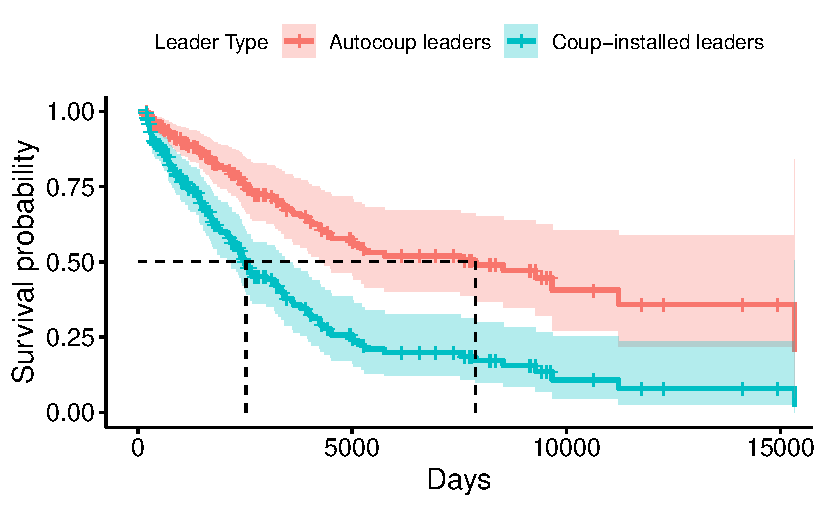
\includegraphics{leader_survival_CPS_files/figure-pdf/fig-coxSurv-1.pdf}

}

\subcaption{\label{fig-coxSurv-1}Cox PH Model}

\end{minipage}%
%
\begin{minipage}{0.50\linewidth}

\centering{

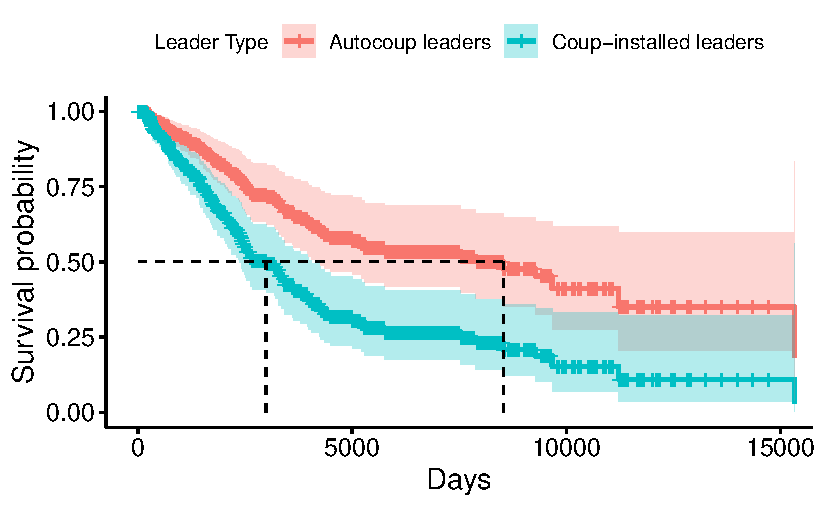
\includegraphics{leader_survival_CPS_files/figure-pdf/fig-coxSurv-2.pdf}

}

\subcaption{\label{fig-coxSurv-2}Time-dependent Cox Model}

\end{minipage}%

\caption{\label{fig-coxSurv}Survival curves for Cox Model}

\end{figure}%

The survival curves in Figure~\ref{fig-coxSurv} displays the survival
rates for both types of leaders, highlighting the differences in their
survival curves. Both the Cox PH model and the time-dependent Cox model
yield similar results. Notably, the survival curve for coup-installed
leaders has a significantly lower trajectory than that of autocoup
leaders. The steeper drop at the early stage for coup-installed leaders
indicates they are more likely to be ousted shortly after assuming
power. Additionally, the survival curve for coup-installed leaders
crosses the median survival line much earlier (about 3,000 days) than
that of autocoup leaders (about 8,500 days). This disparity suggests
that autocoup leaders tend to remain in power for longer durations than
their coup-installed counterparts.

\begin{figure}

\begin{minipage}{0.50\linewidth}

\centering{

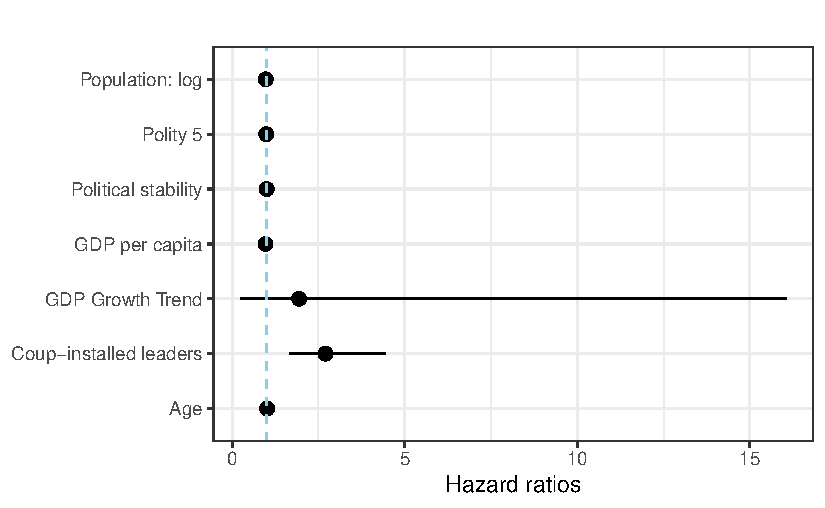
\includegraphics{leader_survival_CPS_files/figure-pdf/fig-coxHR-1.pdf}

}

\subcaption{\label{fig-coxHR-1}Cox PH Model}

\end{minipage}%
%
\begin{minipage}{0.50\linewidth}

\centering{

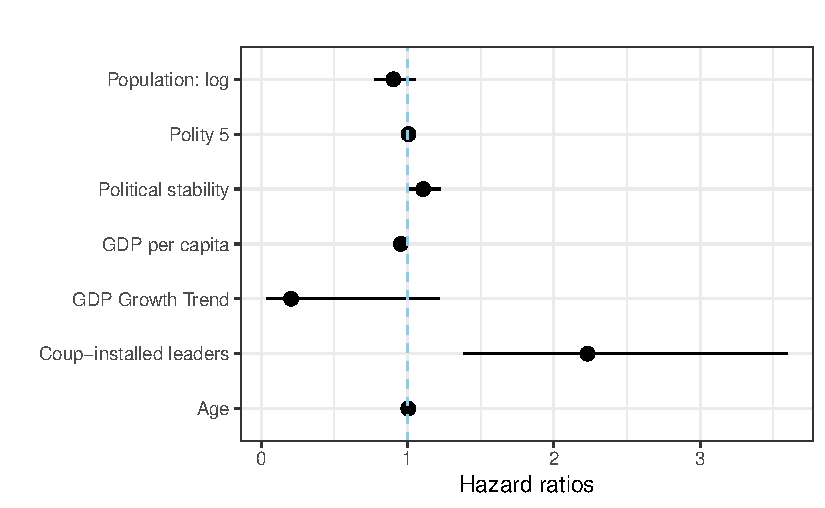
\includegraphics{leader_survival_CPS_files/figure-pdf/fig-coxHR-2.pdf}

}

\subcaption{\label{fig-coxHR-2}Time-dependent Cox Model}

\end{minipage}%

\caption{\label{fig-coxHR}Hazard ratios and 95\% CIs for Leader Ousting}

\end{figure}%

Figure~\ref{fig-coxHR} displays the hazard ratios and corresponding 95\%
confidence intervals for the variables incorporated in the Cox model.
Both the Cox Proportional Hazards (PH) model and the time-dependent
model produce similar plots, reinforcing the robustness of the findings.
Key points to note include:

\begin{itemize}
\item
  The closer the hazard ratio (represented by the dots) is to 1, the
  less impact the variable has on the risk of being ousted. A hazard
  ratio of 1 indicates no effect.
\item
  The whiskers extending from the dots represent the 95\% confidence
  intervals. If these whiskers cross the vertical blue line at 1, it
  indicates that the variable is not statistically significant at the
  5\% level.
\item
  The hazard ratio for coup-installed leaders is significantly greater
  than 1 and statistically significant at the 5\% level. This indicates
  that coup-installed leaders face a substantially higher risk of being
  ousted compared to autocoup leaders.
\item
  Most other variables have hazard ratios close to 1, suggesting that a
  one-unit increase in these variables does not significantly affect the
  risk of being ousted.
\item
  Although the hazard ratio for GDP growth trend is considerably less
  than 1 in the time-dependent model, indicating a potential protective
  effect, it is not statistically significant at the 5\% level. However,
  it is statistically significant at the 10\% level, suggesting that
  better economic performance may help to consolidate the rule of the
  incumbents to some extent, albeit the evidence is not as strong.
\end{itemize}

\subsection{Assessing the proportional hazards
assumption}\label{assessing-the-proportional-hazards-assumption}

Assessing the proportional hazards assumption is crucial for the
validity of the Cox model results. To evaluate this, we used the
chi-square test based on Schoenfeld residuals to determine whether the
covariate effects remain constant (proportional) over time. Although the
Cox PH model violates the proportional hazards assumption, our primary
analysis relies on the time-dependent Cox model, which does not show
strong evidence of violating the proportional hazards assumption for any
covariate. The global p-value of 0.416 is much greater than the 5\%
significance level, indicating that the proportional hazards assumption
is reasonably met for the time-dependent Cox model.

\section{Conclusion}\label{conclusion}

This study explores the survival durations of political leaders who come
to power through unconventional means, specifically focusing on coups
and autocoups. Based on the hypothesis that the mode of accession
affects leader tenure, I use survival analysis techniques, including the
Cox proportional hazards model and a time-dependent Cox model, to
investigate this phenomenon. The findings suggest that autocoup leaders
tend to have longer tenures than coup-installed leaders.

Empirical analysis reveals a significant disparity in tenure length:
leaders who assume power via autocoup remain in office for an average of
11 years, compared to just 5.6 years for those installed by coups.
Moreover, the time-dependent Cox model indicates that coup-installed
leaders are 2.23 times more likely to be ousted from power at any given
time compared to their autocoup counterparts, all other factors being
equal. These findings underscore the importance of understanding the
autocoup as a mechanism through which leaders extend their rule by
manipulating legal frameworks and weakening institutional constraints.

The implications of these findings are profound. The relative ease and
potential rewards of an autocoup could incentivize more leaders to
resort to this method of power retention, particularly in fragile
democracies or transitioning regimes. Consequently, democratic
backsliding may become more prevalent, as autocoups erode democratic
institutions and undermine constitutional norms.

This study contributes significantly to the literature on political
leadership survival by showing that the mode of accession has a
substantial impact on leader tenure, an aspect that has received limited
attention in previous research. Methodologically, this work advances the
field by applying robust survival analysis techniques, including both
Cox models, to provide a nuanced understanding of the dynamics that
influence leadership stability.

However, the study is not without limitations. The analysis relies on an
autocoup dataset that was collected and coded by the author, a
relatively novel concept in the academic sphere. As the understanding
and recognition of ``autocoup'' as a term continue to evolve, future
research should refine and expand the dataset. Incorporating additional
cases and cross-referencing with other forms of irregular leadership
transitions would contribute to a more comprehensive view of political
survival under such conditions.

In conclusion, this study highlights the need for more refined
approaches to studying political tenure and irregular power retention.
By offering valuable insights into the dynamics of political stability
and the risks associated with non-democratic leadership transitions,
this research emphasizes the importance of continued investigation into
the complex relationships between power, legitimacy, and survival in
political leadership.

\newpage

\section*{References}\label{references}
\addcontentsline{toc}{section}{References}

\phantomsection\label{refs}
\begin{CSLReferences}{1}{0}
\bibitem[\citeproctext]{ref-arriola2009}
Arriola, Leonardo R. 2009. {``Patronage and Political Stability in
Africa.''} \emph{Comparative Political Studies} 42 (10): 1339--62.
\url{https://doi.org/10.1177/0010414009332126}.

\bibitem[\citeproctext]{ref-bomprezzi2024wedded}
Bomprezzi, Pietro, Axel Dreher, Andreas Fuchs, Teresa Hailer, Andreas
Kammerlander, Lennart Kaplan, Silvia Marchesi, Tania Masi, Charlotte
Robert, and Kerstin Unfried. 2024. {``Wedded to Prosperity? Informal
Influence and Regional Favoritism.''} Discussion Paper. CEPR.

\bibitem[\citeproctext]{ref-buenodemesquita2003}
Bueno de Mesquita, Bruce, Alastair Smith, Randolph M. Siverson, and
James D. Morrow. 2003. \emph{The Logic of Political Survival}. The MIT
Press. \url{https://doi.org/10.7551/mitpress/4292.001.0001}.

\bibitem[\citeproctext]{ref-davenport2021}
Davenport, Christian, Babak RezaeeDaryakenari, and Reed M Wood. 2021.
{``Tenure Through Tyranny? Repression, Dissent, and Leader Removal in
Africa and Latin America, 1990{\textendash}2006.''} \emph{Journal of
Global Security Studies} 7 (1).
\url{https://doi.org/10.1093/jogss/ogab023}.

\bibitem[\citeproctext]{ref-debruin2020}
De Bruin, Erica. 2020. {``Preventing Coups d{'}état.''} In, 1--12.
Cornell University Press.
\url{https://doi.org/10.7591/cornell/9781501751912.003.0001}.

\bibitem[\citeproctext]{ref-easton2018}
Easton, Malcolm R, and Randolph M Siverson. 2018. {``Leader Survival and
Purges After a Failed Coup d{'}état.''} \emph{Journal of Peace Research}
55 (5): 596--608. \url{https://doi.org/10.1177/0022343318763713}.

\bibitem[\citeproctext]{ref-escribuxe0-folch2013}
Escribà-Folch, Abel. 2013. {``Repression, Political Threats, and
Survival Under Autocracy.''} \emph{International Political Science
Review} 34 (5): 543--60. \url{https://doi.org/10.1177/0192512113488259}.

\bibitem[\citeproctext]{ref-fariss2022}
Fariss, Christopher J., Therese Anders, Jonathan N. Markowitz, and
Miriam Barnum. 2022. {``New Estimates of Over 500 Years of Historic GDP
and Population Data.''} \emph{Journal of Conflict Resolution} 66 (3):
553--91. \url{https://doi.org/10.1177/00220027211054432}.

\bibitem[\citeproctext]{ref-frantz2016}
Frantz, Erica, and Elizabeth A. Stein. 2016. {``Countering Coups:
Leadership Succession Rules in Dictatorships.''} \emph{Comparative
Political Studies} 50 (7): 935--62.
\url{https://doi.org/10.1177/0010414016655538}.

\bibitem[\citeproctext]{ref-gandhi2007}
Gandhi, Jennifer, and Adam Przeworski. 2007. {``Authoritarian
Institutions and the Survival of Autocrats.''} \emph{Comparative
Political Studies} 40 (11): 1279--1301.
\url{https://doi.org/10.1177/0010414007305817}.

\bibitem[\citeproctext]{ref-gassebner2016}
Gassebner, Martin, Jerg Gutmann, and Stefan Voigt. 2016. {``When to
Expect a Coup d{'}état? An Extreme Bounds Analysis of Coup
Determinants.''} \emph{Public Choice} 169 (3-4): 293--313.
\url{https://doi.org/10.1007/s11127-016-0365-0}.

\bibitem[\citeproctext]{ref-goemans2009}
Goemans, Henk E., Kristian Skrede Gleditsch, and Giacomo Chiozza. 2009.
{``Introducing Archigos: A Dataset of Political Leaders.''}
\emph{Journal of Peace Research} 46 (2): 269--83.
\url{https://doi.org/10.1177/0022343308100719}.

\bibitem[\citeproctext]{ref-krishnarajan2019}
Krishnarajan, Suthan. 2019. {``Economic Crisis, Natural Resources, and
Irregular Leader Removal in Autocracies.''} \emph{International Studies
Quarterly} 63 (3): 726--41. \url{https://doi.org/10.1093/isq/sqz006}.

\bibitem[\citeproctext]{ref-licht2009}
Licht, Amanda A. 2009. {``Coming into Money: The Impact of Foreign Aid
on Leader Survival.''} \emph{Journal of Conflict Resolution} 54 (1):
58--87. \url{https://doi.org/10.1177/0022002709351104}.

\bibitem[\citeproctext]{ref-marshall2005current}
Marshall, Monty G. 2005. {``Current Status of the World's Major Episodes
of Political Violence.''} \emph{Report to Political Instability Task
Force.(3 February)}.

\bibitem[\citeproctext]{ref-morrison2009}
Morrison, Kevin M. 2009. {``Oil, Nontax Revenue, and the
Redistributional Foundations of Regime Stability.''} \emph{International
Organization} 63 (1): 107--38.
\url{https://doi.org/10.1017/s0020818309090043}.

\bibitem[\citeproctext]{ref-palmer1999}
Palmer, Harvey D., and Guy D. Whitten. 1999. {``The Electoral Impact of
Unexpected Inflation and Economic Growth.''} \emph{British Journal of
Political Science} 29 (4): 623--39.
\url{https://doi.org/10.1017/s0007123499000307}.

\bibitem[\citeproctext]{ref-powell2017}
Powell, Jonathan. 2017. {``Leader Survival Strategies and the Onset of
Civil Conflict: A Coup-Proofing Paradox.''} \emph{Armed Forces \&
Society} 45 (1): 27--44. \url{https://doi.org/10.1177/0095327x17728493}.

\bibitem[\citeproctext]{ref-powell2011}
Powell, and Thyne. 2011. {``Global Instances of Coups from 1950 to 2010:
A New Dataset.''} \emph{Journal of Peace Research} 48 (2): 249--59.
\url{https://doi.org/10.1177/0022343310397436}.

\bibitem[\citeproctext]{ref-quirozflores2012}
Quiroz Flores, Alejandro, and Alastair Smith. 2012. {``Leader Survival
and Natural Disasters.''} \emph{British Journal of Political Science} 43
(4): 821--43. \url{https://doi.org/10.1017/s0007123412000609}.

\bibitem[\citeproctext]{ref-smith2004}
Smith, Benjamin. 2004. {``Oil Wealth and Regime Survival in the
Developing World, 1960{\textendash}1999.''} \emph{American Journal of
Political Science} 48 (2): 232--46.
\url{https://doi.org/10.1111/j.0092-5853.2004.00067.x}.

\bibitem[\citeproctext]{ref-sudduth2017}
Sudduth, Jun Koga. 2017. {``Strategic Logic of Elite Purges in
Dictatorships.''} \emph{Comparative Political Studies} 50 (13):
1768--1801. \url{https://doi.org/10.1177/0010414016688004}.

\bibitem[\citeproctext]{ref-sudduth2018}
Sudduth, Jun Koga, and Curtis Bell. 2018. {``The Rise Predicts the Fall:
How the Method of Leader Entry Affects the Method of Leader Removal in
Dictatorships.''} \emph{International Studies Quarterly} 62 (1):
145--59. \url{https://doi.org/10.1093/isq/sqx075}.

\bibitem[\citeproctext]{ref-svolik2014}
Svolik, Milan W. 2014. {``Which Democracies Will Last? Coups, Incumbent
Takeovers, and the Dynamic of Democratic Consolidation.''} \emph{British
Journal of Political Science} 45 (4): 715--38.
\url{https://doi.org/10.1017/s0007123413000550}.

\bibitem[\citeproctext]{ref-survival}
Therneau, Terry M. 2024. {``A Package for Survival Analysis in r.''}
\url{https://CRAN.R-project.org/package=survival}.

\bibitem[\citeproctext]{ref-thyne2017}
Thyne, Clayton, Powell, Sarah Parrott, and Emily VanMeter. 2017. {``Even
Generals Need Friends.''} \emph{Journal of Conflict Resolution} 62 (7):
1406--32. \url{https://doi.org/10.1177/0022002716685611}.

\bibitem[\citeproctext]{ref-williams2011}
Williams, Laron K. 2011. {``Pick Your Poison: Economic Crises,
International Monetary Fund Loans and Leader Survival.''}
\emph{International Political Science Review} 33 (2): 131--49.
\url{https://doi.org/10.1177/0192512111399006}.

\bibitem[\citeproctext]{ref-wright2008}
Wright, Joseph. 2008. {``To Invest or Insure?''} \emph{Comparative
Political Studies} 41 (7): 971--1000.
\url{https://doi.org/10.1177/0010414007308538}.

\bibitem[\citeproctext]{ref-wright2013}
Wright, Joseph, Erica Frantz, and Barbara Geddes. 2013. {``Oil and
Autocratic Regime Survival.''} \emph{British Journal of Political
Science} 45 (2): 287--306.
\url{https://doi.org/10.1017/s0007123413000252}.

\bibitem[\citeproctext]{ref-yu2016}
Yu, Shu, and Richard Jong-A-Pin. 2016. {``Political Leader Survival:
Does Competence Matter?''} \emph{Public Choice} 166 (1-2): 113--42.
\url{https://doi.org/10.1007/s11127-016-0317-8}.

\bibitem[\citeproctext]{ref-zhu2024}
Zhu, Qi. 2024. {``Leadership Transitions and Survival: Coups, Autocoups,
and Power Dynamics.''} PhD thesis, University of Essex.

\end{CSLReferences}




\end{document}
